\documentclass[12pt]{report}

%%%%%%%%%%%%%%%%%%%%%%%%%%%%%%%%%%%%%%%%%%%%%%%%%%%%%%%%%%%%%%%%%%%%
% package and document formatting stuff
%%%%%%%%%%%%%%%%%%%%%%%%%%%%%%%%%%%%%%%%%%%%%%%%%%%%%%%%%%%%%%%%%%%%

% symbols and math stuff
\usepackage{amsmath,amsthm,amssymb}
\usepackage{tikz}
\usepackage{tkz-graph}
\usetikzlibrary{arrows,%
                petri,%
                topaths}%

\usepackage{tkz-berge}


% math operators
\usepackage{amsopn}

% script and caligraphics
\usepackage{eucal,mathrsfs}

% indexing
\usepackage{makeidx}

\usepackage{enumerate}

% formatting
\usepackage{fullpage}

% links and colors
\usepackage{color}
\usepackage[pdfstartview=FitH,
%             pdfauthor={\myauthor},
%             pdftitle={\mytitle},
            colorlinks,
            linkcolor=reference,
            citecolor=citation,
            urlcolor=e-mail,
            backref]{hyperref}
\usepackage[all]{xy}

\definecolor{todo}{rgb}{.80,.20,.20}
\definecolor{e-mail}{rgb}{0,.40,.80}
\definecolor{reference}{rgb}{.10,.40,.42}
\definecolor{mrnumber}{rgb}{.80,.40,0}
\definecolor{citation}{rgb}{0,.40,.80}

\usepackage{graphicx}

%%%%%%%%%%%%%%%%%%%%%%%%%%%%%%%%%%%%%%%%%%%%%%%%%%%%%%%%%%%%%%%%%%%%
% theorem stuff
%%%%%%%%%%%%%%%%%%%%%%%%%%%%%%%%%%%%%%%%%%%%%%%%%%%%%%%%%%%%%%%%%%%%

\theoremstyle{plain}

\newtheorem{thm}{Theorem}[section]
\newtheorem{defn}[thm]{Definition}
\newtheorem{deflem}[thm]{Definition/Lemma}
\newtheorem{notn}[thm]{Notation}
\newtheorem{convention}[thm]{Convention}
\newtheorem{lem}[thm]{Lemma}
\newtheorem{aside}[thm]{Aside}
\newtheorem{rem}[thm]{Remark}
\newtheorem{ex}[thm]{Example}
\newtheorem{facts}[thm]{Facts}
\newtheorem{cor}[thm]{Corollary}
\newtheorem{conj}[thm]{Conjecture}
\newtheorem{prop}[thm]{Proposition}

\newtheorem{question}[thm]{Question}
\newtheorem{exercise}{Exercise}[section]

%%%%%%%%%%%%%%%%%%%%%%%%%%%%%%%%%%%%%%%%%%%%%%%%%%%%%%%%%%%%%%%%%%%%
% typography stuff
%%%%%%%%%%%%%%%%%%%%%%%%%%%%%%%%%%%%%%%%%%%%%%%%%%%%%%%%%%%%%%%%%%%%

\newcommand{\mb}[1]{\mathbf #1}
\newcommand{\mbb}[1]{\mathbb #1}
\newcommand{\mf}[1]{\mathfrak #1}
\newcommand{\mc}[1]{\mathcal #1}
\newcommand{\ms}[1]{\mathscr #1}
\newcommand{\mcu}[1]{\mathcu #1}
\newcommand{\oper}[1]{\operatorname{#1}}

\newcommand{\da}{\downarrow}
\newcommand{\ra}{\rightarrow}
\newcommand{\hra}{\hookrightarrow}
\newcommand{\dra}{\dashrightarrow}
\newcommand{\la}{\leftarrow}
\newcommand{\lra}{\longrightarrow}

\newcommand{\ov}{\overline}
\newcommand{\til}{\widetilde}
\newcommand{\wh}{\widehat}

\newcommand{\ZZ}{\mathbb{Z}}

\newcommand{\lcm}{\oper{lcm}}

%%%%%%%%%%%%%%%%%%%%%%%%%%%%%%%%%%%%%%%%%%%%%%%%%%%%%%%%%%%%%%%%%%%%
% other stuff
%%%%%%%%%%%%%%%%%%%%%%%%%%%%%%%%%%%%%%%%%%%%%%%%%%%%%%%%%%%%%%%%%%%%

\newcommand{\todo}[1]{\textcolor{todo}{#1}}

%%%%%%%%%%%%%%%%%%%%%%%%%%%%%%%%%%%%%%%%%%%%%%%%%%%%%%%%%%%%%%%%%%%%
% end preamble
%%%%%%%%%%%%%%%%%%%%%%%%%%%%%%%%%%%%%%%%%%%%%%%%%%%%%%%%%%%%%%%%%%%%

\begin{document}

%%%%%%%%%%%%%%%%%%%%%%%%%%%%%%%%%%%%%%%%%%%%%%%%%%%%%%%%%%%%%%%%%%%%
% title stuff
%%%%%%%%%%%%%%%%%%%%%%%%%%%%%%%%%%%%%%%%%%%%%%%%%%%%%%%%%%%%%%%%%%%%


\author{Daniel Krashen}
\title{Notes on Signal Processing\\Discrete Fourier and Wavelet Transforms}
\date{\today}

\maketitle
\tableofcontents

%%%%%%%%%%%%%%%%%%%%%%%%%%%%%%%%%%%%%%%%%%%%%%%%%%%%%%%%%%%%%%%%%%%%
% document stuff
%%%%%%%%%%%%%%%%%%%%%%%%%%%%%%%%%%%%%%%%%%%%%%%%%%%%%%%%%%%%%%%%%%%%

\iffalse
\chapter*{Version Notes}
\addcontentsline{toc}{chapter}{Version Notes}
\fi

\iffalse
\section{Updates 1/25/2020}
\begin{itemize}
\item Nothing to say, but generally update information would go here.
\item e.g. added stuff to Section~\ref{lecture 1}
\end{itemize}
\fi

\chapter{The Discrete Fourier Transform}

The discrete Fourier transform is a tool to go between describing a sampled, periodic signal as a list of measurements and describing it as a combination of basic waveforms.

\section{Periodic signals and their representations}

\subsection{Periodic signals as vectors}

We start by imagining we have a periodic signal $f$, which we sample at a times $0, 1, 2, N-1$. We denote these measurements as
\[ f[0], f[1], f[2], \ldots, f[N-1]. \]
We assume that the signal is periodic with period $N$, so that the value at $N$ agrees with the value at $0$, the value at $N+1$ agrees with the value at $1$, etc. That is, we have $f[N] = f[0]$, and more generally $f[k + N] = f[k]$ for all $k$.

We may write this information as a vector
\[
\vec f =
\left[
\begin{matrix}
f[0] \\
f[1] \\
\vdots \\
f[N-1]
\end{matrix}
\right]
\]

That is, if we write $f$ for the sampled period signal, we will write $\vec f$ for the vector whose coordinates are the values sampled.
Implicitly, in doing this, we are regarding these (sampled periodic) signals themselves as forming a vector space, and we have chosen a basis of such signals. Explicitly, when we write

\begin{align*}
\vec f =
\left[
\begin{matrix}
f[0] \\
f[1] \\
\vdots \\
f[N-1]
\end{matrix}
\right]
&=
f[0]
\left[
\begin{matrix}
1 \\
0 \\
\vdots \\
0 \\
0
\end{matrix}
\right]
+
f[1]
\left[
\begin{matrix}
0 \\
1 \\
\vdots \\
0 \\
0
\end{matrix}
\right]
+
\cdots
+
f[N-1]
\left[
\begin{matrix}
0 \\
0 \\
\vdots \\
0 \\
1
\end{matrix}
\right] \\
\end{align*}
we think of this as corresponding to the equation
\[f = f[0]e_0 + f[1] e_1 + \cdots f[N-1]e_{N-1}\\
= \sum_{k = 0}^{N-1} f[k] e_k,
\]
where the signal $e_k$ has values described by
\[ e_k[j] = 0 \text{ if $k \neq j$, and } e_k[k] = 1. \]

\begin{notn}
We remark that, unlike conventional notation we index our vectors (and later our matrices), starting with the index of $0$ (as in computer science).
\end{notn}

\subsection{The wave basis for periodic signals}

Let us introduce the basic ``wave functions'' which we will use to describe our signals. These special periodic signals are described as complex number of unit length, that rotate about the origin at a constant rate.

That is, such a wave function $E$ will be determined by an angle $\theta$, and when measured at time $j$, yields a complex number of unit length, making an angle of $j\theta$ in the counterclockwise direction with the positive $x$-axis, as shown in Figure~\ref{jtheta}.

\begin{figure}[ht!]
\centering
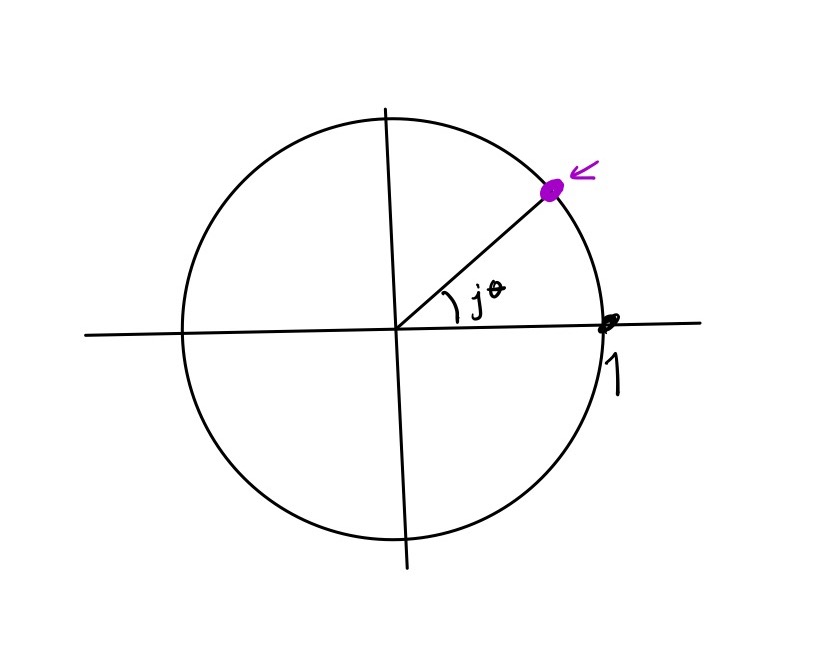
\includegraphics[width=90mm]{jtheta.jpg}
\caption{unit complex number at angle $j \theta$ \label{jtheta}}
\end{figure}

As described in Chapter~\ref{complex exponentials}, we may represent this complex number as
\[E[j] = e^{ij\theta} = \cos{j\theta} + i \sin{j \theta}.\]

Of course, since we are interested in periodic signals, we will require that $N\theta$ is a multiple of $2\pi$. We therefore have the following natural choices for $\theta$:
\[\theta = 0, 2 \pi/N, 4 \pi / N, \ldots, 2k\pi/N, \ldots, 2(N-1)\pi/N.\]
Note that it would serve no purpose to continue, as $2N\pi/N = 2\pi$ also corresponds to an angle of $0$.

We can represent these periodic signals as follows. Setting $E_k$ to be the signal with $\theta= 2k\pi/N$, we have:
\[E_k[j] = e^{ij\theta} = e^{ij2k\pi/N} = \left(e^{2\pi i / N}\right)^{jk}. \]
For convenience, we let $\omega = e^{2 \pi i / N}$, so that we may write our basic waveforms as:
\[E_k[j] = \omega^{jk} \]

The critical fact about these signals is that they also form a basis for the vector space of our periodic signals. That is, just as we may uniquely represent a signal $f$ as a linear combination of the signals $e_k$, we may also uniquely represent it is a linear combination of the signals $E_k$ as well. The change of basis matrix has a particularly nice form. It turns out to be equal to $1/N F_N$, where $F_N$ is the ``Fourier'' matrix. It's entries are given by $(F_N)_{k,j} = \omega^{-jk}$. That is, if we write $f = \sum f[k] e_k$, and do the matrix product:
\[
F_N
\left[
\begin{matrix}
	f[0] \\
	f[1] \\
	\vdots \\
	f[N-1]
\end{matrix}
\right]
=
\left[
\begin{matrix}
	\hat f[0] \\
	\hat f[1] \\
	\vdots \\
	\hat f[N-1]
\end{matrix}
\right]
\]

Then the coefficients $\hat f[k]$ of the resulting vector, which are called the \textbf{Fourier coefficients} of $f$, are related to expressing $f$ in terms of the basic waveforms as follows:
\begin{equation} \label{fourier basis expression}
f = \sum_k f[k] e_k = \sum \frac 1 N \hat f[k] E_k.
\end{equation}

The matrix $F_N$ (or rather the corresponding linear transformation) is called \textbf{Discrete Fourier Transform}, and the vector
\[\vec{\hat f} = F_N \vec f =
\left[
\begin{matrix}
	\hat f[0] \\
	\hat f[1] \\
	\vdots \\
	\hat f[N-1]
\end{matrix}
\right]
\]
is called the Fourier transform of $\vec f$. Note that since the Fourier coefficients are obtain by the application of a linear transformation, they satisfy
\begin{equation} \label{hat is linear}
\widehat{f + g}[k] = \hat f[k] + \hat g[k] \text{, and }\widehat{\lambda f}[k] = \lambda \hat f[k]
\end{equation}
for scalars $\lambda$.

\medskip
Let us work out the effect of this Fourier transform in some examples, starting with the standard basis signals $e_k$.
As the $k$'th column of the matrix $F_N$ represents the effect of the Fourier tranform on the $k$'th basis vector $\vec e_k$, we find that $F_N \vec e_k$ is represented by the column vector $\begin{bmatrix} \omega^{0} \\ \omega^{-k} \\ \omega^{-2k} \\ \vdots \\ \omega^{-(N-1)k} \end{bmatrix}$. Since by definition, these entries are the Fourier coefficients $\hat e_k[j]$, we find the useful fact:
\begin{equation} \label{fourier coeffs of std}
\boxed{\hat e_k[j] = \omega^{-jk}}
\end{equation}
Using Equation~\ref{fourier coeffs of std} and Equation~\ref{hat is linear}, we can give a formula for the Fourier coefficients of a general signal $f = \sum_k f[k] e_k$. For this, we obtain:
\begin{equation*}
\hat f[j] = \widehat{\left(\sum_k f[k] e_k\right)}[j] = \sum_k f[k] \hat e_k[j] = \sum_k f[k] \omega^{-jk}
\end{equation*}
and so
\begin{equation} \label{fourier coeffs formula}
\boxed{\hat f[j] = \sum_k f[k] \omega^{-jk}}
\end{equation}
Finally, let us compute the Fourier coefficients of the standard wave functions. For this, we will simply use the definition of the Fourier coefficients, and their relation to the change of basis. We have, by applying Equation~\ref{fourier basis expression} in the case $f = E_j$:
\begin{align*}
E_j &= \sum_k \frac{\hat E_j[k]}{N} E_k \\
&= \frac{\hat E_j[0]}{N} E_0 + \cdots +
\frac{\hat E_j[j-1]}{N} E_{j-1} + \frac{\hat E_j[j]}{N} E_{j} + \frac{\hat E_j[j+1]}{N} E_{j+1} + \cdots + \frac{\hat E_j[N-1]}{N} E_{N-1}
\end{align*}
But of course we can also write (trivially):
\begin{align*}
E_j &= 0 \cdot E_0 + \cdots +
0 \cdot E_{j-1} + 1 \cdot E_{j} + 0 \cdot E_{j+1} + \cdots + 0 \cdot E_{N-1}
\end{align*}

But since the signals $E_k$ form a basis, the expression for $E_j$ as a combination of the $E_k$'s is unique. Equating these gives:
\begin{equation} \label{fourier coeffs of waveforms}
\boxed{\hat E_j[k] = 0 \text{, if $k \neq j$, and } \hat E_j[j] = N}
\end{equation}

\section{Filters, circular convolution and circulant matrices}

\section{The fast Fourier transform}

\appendix

\chapter{Complex exponentials}

\section{Complex arithmetic and polar form}

Although in typical applications, we deal with real numbers (to some fixed precision), allowing ourselves to work also with complex number can add a great variety of additional tools to bring to bear. In particular, we will eventually see that periodic functions, such as the sine and cosine, can be efficiently and compactly described via complex exponential functions, and doing this makes it a great deal more efficient decompose periodic signals into basic waveforms (i.e. via the Fourier transform).

Recall that a complex number $z = x + iy$, can be thought of graphically as a point in the complex plane, where we think of $x$ and $y$ as the coordinates of a point $(x, y)$. In this representation, it is clear that addition of complex numbers corresponds to addition of vectors -- that is
\[ (x_1 + i y_1) + (x_2 + i y_2) = (x_1 + x_2) + i (y_1 + y_2)\]
agrees with the vector sum
\[ (x_1, y_1) + (x_2, y_2) = (x_1 + x_2, y_1 + y_2) \]
But what about complex multiplication? For multiplication we see a nice visual interpretation by considering a polar representation of the complex number: if the point $(x_j, y_j)$, $j = 1, 2$ in the plane correpsonds to a vector of length $r_j$ and making an angle of $\theta_j$ with the positive $x$-axis, then we may write
\[z_j = x_j + i y_j = r_j \cos \theta_j + i r_j \sin \theta_j \]
and we find (using the sum formula for sine and cosine):

\begin{align} \label{angles add}
(x_1 + i y_1)(x_2 + i y_2) &= (r_1 \cos \theta_1 + i r_1 \sin \theta_1)(r_2 \cos \theta_2 + i r_2 \sin \theta_2) \\ &= r_1 r_2 \Big( (\cos \theta_1 \cos \theta_2 - \sin \theta_1 \sin \theta_2) (\cos \theta_1 \sin \theta_2 + \cos \theta_2 \sin \theta_1 )\Big) \\ &= r_1 r_2 \cos (\theta_1 + \theta_2) + i r_1 r_2 \sin (\theta_1 + \theta_2).
\end{align}

Said another way, we can visualize the multiplication of complex numbers in the following way: \textbf{lengths multiply and angles add}.

\section{Complex Exponentials} \label{complex exponentials}

We can view complex multiplication in a more intuitive light with the aid of Euler's formula, which gives a relationship between the complex exponential function and the polar representation of a complex number. Euler's formula states that for a real number\footnote{in fact the formula holds for complex numbers as well, and can be taken as a definition of cosine and sine for complex arguments} $\theta$, we have
\[e^{i \theta} = \cos \theta + i \sin \theta. \]
This formula can be verified by, for example, replacing each side by the corresponding power series expansions.

The complex exponential function -- that is, the function $e^z$ where $z$ can be any complex number, shares the usual familar properties with its real counterpart: $e^{z + w} = e^z e^w$, immediately giving again the multiplication rule from equation~\ref{angles add} above.

\iffalse
Let's visualize how the graph of the function $e^{i \theta}$ as a function of the real variable $\theta$.
\fi

\iffalse
Given a complex number, expressed as \[z = r \cos \theta + i r \sin \theta,\] we see that we can raise $z$ to positive integer powers by the formula
\[z^n = r^n \cos n\theta + i r^n \sin n\theta.\]
In particular, it makes sense to extend this definition and simply define the exponential $z^s$ for any real number $s$, by the formula
\[z^s = r^s \cos s\theta + i r^s \sin s\theta\]
\fi

\section{Roots of unity}

%\bibliographystyle{alpha}
%\bibliography{citations}
\printindex

\end{document}
